\newpage
\subsubsection{Swellpro SplashDrone 4}
\begin{wrapfigure}{r}{0.3\textwidth}
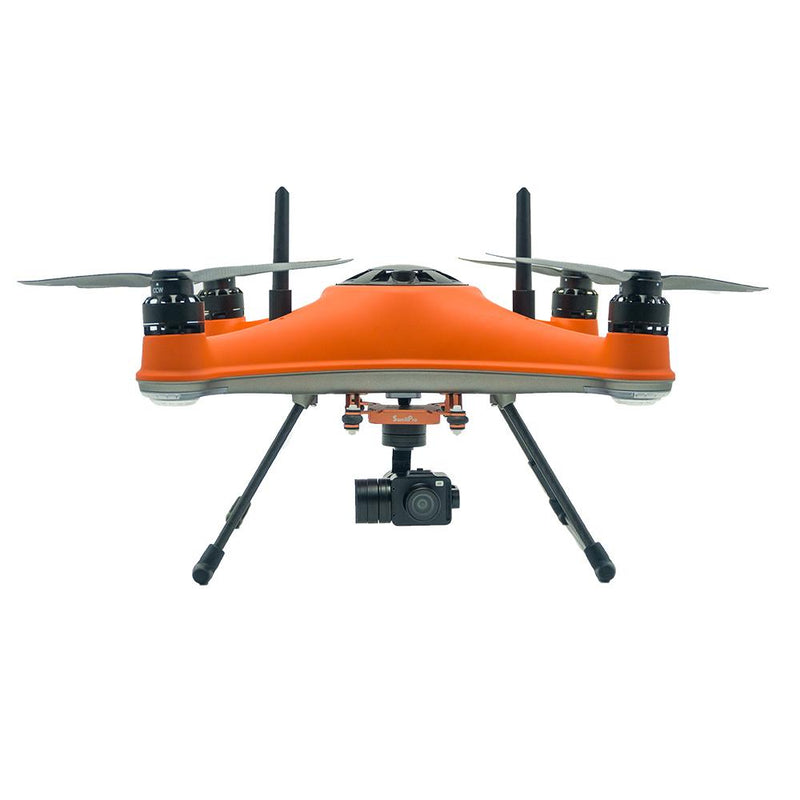
\includegraphics[width=1\linewidth]{uav/models/01_splashdrone4.png}
\caption{SplashDrone 4}
\end{wrapfigure}
The SplashDrone 4 \cite{splashdrone4} is Swellpro's flagship drone. It is fully designed to be used in the water.

\paragraph{Payload capacity}\mbox{Score: 1.5} \\
The payload capacity of the SplashDrone 4 is 2kg, enough for all of our gear.

\paragraph{Mounting clearance}\mbox{Score: 1.3} \\
The SplashDrone 4 is a medium compact drone and therefore doesn't have a lot of clearance for sensors. It does have mounting holes for payloads at the bottom of the drone, which make mounting sensors easy. The drone can also flip over in the water, so one could also manually mount sensors on top of the drone. Additionally, Swellpro sells a water collector for the Splashdrone 4 to take water samples. \cite{watercollector}

\paragraph{Navigation/Routing}\mbox{Score: 1.5} \\
One can plan routes for the SplashDrone 4 using the SwellPro SDFly App. The app has support for waypoint mission planning and grid mission planning. Additionally, a SDK and API is also in development for when one wants to create their own add-ons or flight platform.

\paragraph{Flight time}\mbox{Score: 1.5} \\
The flight time of the SplashDrone 4 is 30 minutes, well over the minimum required flight time.

\paragraph{Range}\mbox{Score: 1.5} \\
The maximum radio range is 5.0km, well over the minimum required range. This also includes image transmission.

\paragraph{Waterproof}\mbox{Score: 1.5} \\
The drone is IP67 waterproof, meaning the drone is dust-tight and can immerse up to 1 meter in water. This is well over the minimum required IP rating.

\paragraph{Landing in water}\mbox{Score: 1.5} \\
The drone is designed to land and take off in the water.

\paragraph{Maneuverability}\mbox{Score: 1.4} \\
When the drone turns upside down on the water for any reason, it automatically turns the drone back around to the normal state. It can fly horizontally 10m/s with the GPS being the limiting factor.

\paragraph{Total score:}\mbox{20.7} \\
The SplashDrone 4 seems to be a very adequate system for the project, with it's extensible and water-first design.